\documentclass[a4paper, 12pt]{article}
% math symbols
\usepackage{amssymb}
\usepackage{amsmath}
\usepackage{mathrsfs}
\usepackage[shortlabels]{enumitem}
\usepackage{mathseries}
\usepackage[12pt]{moresize}
\usepackage[style = alphabetic, maxbibnames = 99, backend = biber]{biblatex}
\addbibresource{references.bib}

\usepackage[margin = 2cm]{geometry}

\tolerance = 1000
\emergencystretch = 0.74cm



\pagestyle{empty}
%\parindent = 0mm


\setmathstyle{2020}{Теория информации}{С.А. Лучинин, М.С. Опанасенко}

%\newcommand{\F}{\mathbb{F}}

\newtheorem{problem}{Задача}[section]
\newtheorem{examples}{Задача}[section]
\makeatletter
\renewtcolorbox[use counter = theorem, number within = section]{problem}[1][]{
    enhanced,
    theo = {blue},
    title = {Задача \thetcbcounter\ #1},
    before upper = {\protected@edef\@currentlabel{\csname p@theorem\endcsname\csname thetcbcounter\endcsname}}
}
\makeatother
\makeatletter
\renewtcolorbox[use counter = theorem, number within = section]{examples}[1][]{
    enhanced,
    theo = {blue},
    title = {Пример \thetcbcounter\ #1},
    before upper = {\protected@edef\@currentlabel{\csname p@theorem\endcsname\csname thetcbcounter\endcsname}}
}
\makeatother


%\let\M\undefined
\let\IP\undefined
\newlang{\IP}{\lang{IP}}

\newauthor{ds}{Dmitry}{red!20}

\begin{document}
    \pagestyle{empty}


\begin{tikzpicture}[remember picture, overlay]
    \node[
        shape = rectangle,
        minimum height = \paperheight,
        minimum width = \paperwidth,
        anchor = south west,
        fill = olive!5]
        (sheet) at (current page.south west) {};
    \tikzset{shift = {(sheet.center)}}
    \node at (0, -2) {
        \HUGE
        \begin{tabular}{c}
            \textsc{Теория информации}\\
            \huge Конспект лекций
        \end{tabular}
    };

    \node[inner sep = 0pt, opacity = 0.5] at (6, 10.5){
        
\includegraphics[width = 0.27\textwidth] {pics/sun.png}
    };


    \begin{scope}[shift = {(0, 3)}]
        \node[inner sep = 0pt, opacity = 0.5] at (-5, 0){
            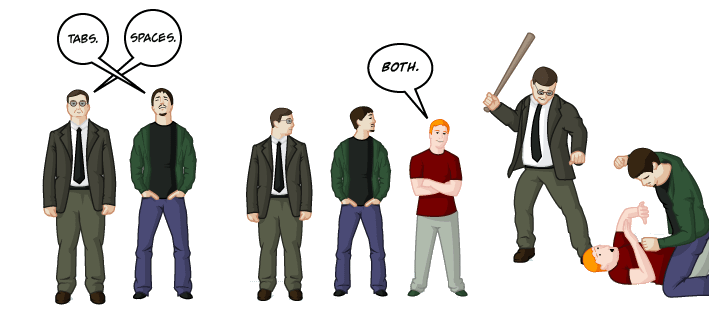
\includegraphics[width = 0.4\textwidth] {pics/tabs-spaces.png}
        };
        \node[inner sep = 0pt, opacity = 0.5] at (-5, -2.3){
            \textsc{Коммуникационная сложность}
        };
        \node[inner sep = 0pt, opacity = 0.5] at (5, 0){
            
\includegraphics[width = 0.4\textwidth] {pics/bender.png}
        };
        \node[inner sep = 0pt, opacity = 0.5] at (5, -2.3){
            \textsc{Колмогоровская сложность}
        };
    \end{scope}

    \begin{scope}[shift = {(0, -8)}]
        \node[inner sep = 0pt, opacity = 0.5] at (0, 0){
            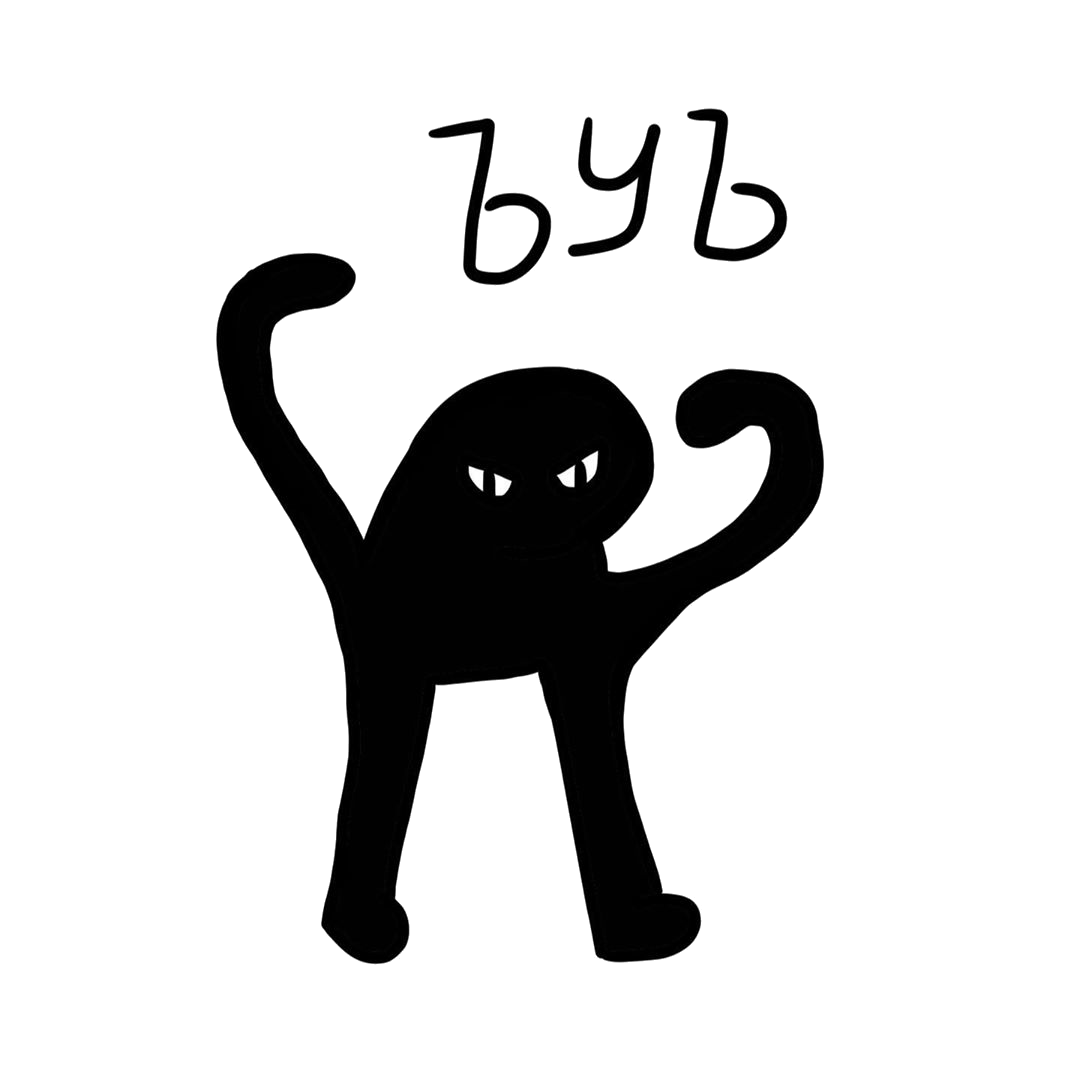
\includegraphics[width = 0.5\textwidth] {pics/uuu.png}
        };
        \node[inner sep = 0pt, opacity = 0.5] at (0, -4.2){
            \textsc{Теория кодирования}
        };
    \end{scope}


%    \pic[scale = 1.6] at (-3.5, -5) {tikzart-gun};

%    \pic[scale = 1.6] at (7, -9) {tikzart-bunny};
%    \pic[scale = 1.6] at (-5, 5) {tikzart-bunny};
%    \pic[scale = 1.6, rotate = 40] at (-5, -8) {tikzart-bunny};
%    \pic[scale = 1.6, rotate = -10, xscale = -1] at (6, 1) {tikzart-bunny};
%    \pic[scale = 1.6, rotate = 30, xscale = -1] at (8, 9) {tikzart-bunny};

%    \draw[platform] (\paperwidth / 2, -12.02) -- ++(-\paperwidth, 0);

%    \foreach \i in {0, 1, ..., 4}{
%        \pic[scale = 4] at (-5 + 1.8 * \i, -12) {tikzart-train};
%        \draw (-3.2 + 1.8 * \i, -11.7) -- ++(-0.2, 0);
%    }
%    \pic[scale = 4] at (-5 + 1.8 * 5, -12) {tikzart-trainhead};
\end{tikzpicture}


\clearpage


    \tableofcontents
    \clearpage
    
    \documentclass[a4paper, 12pt]{article}
% math symbols
\usepackage{amssymb}
\usepackage{amsmath}
\usepackage{mathrsfs}
\usepackage{mathseries}


\usepackage[margin = 2cm]{geometry}

\tolerance = 1000
\emergencystretch = 0.74cm



\pagestyle{empty}
\parindent = 0mm

\renewcommand{\coursetitle}{DM/ML}
\setcounter{curtask}{1}

\setmathstyle{Апрель 2}{Теория информации}{2 курс}


\begin{document}

\libproblem{inf-theory}{entropy-letters}
\libproblem{inf-theory}{find-n}
\libproblem{inf-theory}{volume-3-dim}
\libproblem{inf-theory}{volume-4-dim}
\libproblem{inf-theory}{infinite-word}
\libproblem{inf-theory}{i-dont-know}
\libproblem{inf-theory}{king-poison}
\libproblem{inf-theory}{bounded-entropy}
\libproblem{inf-theory}{prefix-codes}
\libproblem{inf-theory}{prefix-codes-2}

\end{document}



%%% Local Variables:
%%% mode: latex
%%% TeX-master: t
%%% End:

    \section{Информация по Хартли}

\subsection{Базовые свойства}

Пусть дано некоторое множество объектов. Мы хотим ввести некоторую \textit{меру информации}, то есть
хотим понять, сколько информации мы узнаём, получая некоторый элемент данного множества. Одна из
общепринятых мер информации~--- количество бит. Попробуем формализовать эту меру информации

\begin{definition}[Информация по Хартли]
    \label{def:hartley-inf}
	Пусть $A$~--- некоторое конечное множество. За \deftext{информацию в множестве} $A$~--- будем
    принимать следующую величину:
	$$
        \chi(A) \coloneqq \log{\abs{A}}.
    $$
\end{definition}

Данное определение хорошо ложиться на интуитивное представление о том, что необходимо $\log{\abs{A}}$ бит
для описания некоторого элемента множества. Отметим, что число $\chi(A)$ может быть нецелым.
\begin{remark}
	В отличие от курса анализа, под $\log$ мы везде понимаем логарифм по основанию $2$.
\end{remark}

Попробуем описать свойства этого определения.

\begin{proposition}
    Пусть $A \subseteq X \times Y$~--- конечное двумерное множество, $A_X$ --- его проекция на $X$,
    $A_Y$~--- на $Y$. Тогда выполнены следующие свойства: 
	\begin{enumerate}
        \item $\chi(A) \ge 0$;
        \item $\chi(A_X) \le \chi(A)$, $\chi(A_Y) \le \chi(A)$;
        \item $\chi(A) \le \chi(A_X) + \chi(A_Y)$.
    \end{enumerate}
\end{proposition}

\begin{proof}
	Следует из определения.
\end{proof}

Пользуясь этим определением мы можем доказать нетривиальные свойства множеств, например соотношение между
<<объёмом>> и площадями проекций.

\libproblem{inf-theory}{volume-3-dim}

Можем ли мы понять как изменится информация во множестве $A$, если мы уже про него что-то знаем?
Аналогично определению \ref{def:hartley-inf} мы можем описать <<условную информацию>>, содержащуюся в
множестве $A$.

\begin{definition}
	Пусть $A$~--- двумерное множество с проекциями $X$ и $Y$. \deftext{Условную информация} содержащуюся
    в множестве $A$, если мы уже знаем вторую координату, определим следующим образом: 
	$$
        \chi_{Y|X}(A) \coloneqq \max_x{\big(\log|A_x|\big)},
    $$ 
	где $A_x$ --- сечение $A$ по координате $x$.
\end{definition}

Если говорить интуитивно, то эта мера нам описывает достаточное количество бит, нужное для кодирования
элемента, зная его первую проекцию. Существенный недостаток это определения в том, что разным элементам
могут соответствовать сечения разных размеров, а мы этого никак не учитываем.

Нетрудно проверить, что при таком определении выполнено неравенство
$$
    \chi(A) \le \chi(A_Y) + \chi_{X|Y}(A).
$$


В дальнейшем иногда мы будем обозначать множество  $\{1, 2, \dots, n\}$ через $[n]$.

\subsection{Угадывание монетки}

\paragraph{Симметричный вариант.}
Рассмотрим некоторые применения информации по Хартли. Пусть есть два игрока, первый загадывает число от
$1$ до $n$. Сколько вопросов с ответом <<да/нет>> необходимо задать второму игроку, чтобы угадать число?
При этом у задачи есть два варианта: с \textit{неадаптивной} стратегией, когда второй игрок пишет все
вопросы заданы заранее, и \textit{адаптивной} стратегией, когда второй игрок задаёт очередной вопрос,
зная ответы на все предыдущие.  

Для верхней оценки, как в адаптивной, так и не в адаптивной стратегии мы можем предъявить простую
стратегию. Второй игрок может спросить каждый бит числа $n$ в двоичной записи; поэтому количество
запросов не превосходит $h = \lceil \log n \rceil$. Теперь давайте попробуем доказать, что ничего лучше
сделать мы все равно не сможем.
	
Пусть $Q_i$~--- ответ на $i$-ый вопрос (один бит), $N$~--- искомое число,
$$
    B \coloneqq Q_1\times Q_2 \times \cdots \times Q_h.
$$ 

Посмотрим на множество пар $(N, B)$ по всем возможным $N$ и $B$. Корректность протокола означает, что
если мы знаем все $Q_i$, то можем определить число, то есть $\chi_{B}([n]) = 0$. Легко заметить, что
$\chi(Q_i) \leq 1$. Тогда:
$$
    \log{n} \leq \chi(N, B) \leq \sum_{i=1}^{h} \chi(Q_i) + \chi_B([n]) = \sum_{i=1}^{h} \chi(Q_i) \le
    h.
$$
Таким образом, $h \ge \log{n}$, доказана нижняя оценка.
	
Ту же оценку можно было легко получить и другими, более простыми способами, но метод выше обобщается на
гораздо более сложные ситуации.

\paragraph{Асимметричный вариант.}
Немного усложним задачу. Пусть за каждый ответ <<да>> второй игрок платит $1$ монету, а за каждый ответ
<<нет>>~--- 2 монеты.

Давайте попробуем адаптировать нашу стратегию для этого случая. Попробуем запросом делить множество
<<пополам>> с точки зрения стоимости, то есть таким образом, чтобы при ответе <<нет>> мы бы узнавали в
два раза больше информации. (что, например, на первом шаге нам даст следующее соотношение:
$2 \chi_{Q_i = 1}([n]) = \chi_{Q_i = 0}([n])$).

Попробуем понять сколько нам потребуется заплатить при такой стратегии. Пусть $Q_i$~--- ответ на вопрос
<<верно ли, что загаданное число $N$ лежит в множестве $T_i \subseteq X_i$?>>. Пусть $X_i$~--- множество
элементов, в котором может лежать $N$ после первых $i$ вопросов. Наша стратегия говорит, что:
$$
    2 (\chi(X_i) - \chi(T_i)) = \chi(X_i) - \chi(X_i \setminus T_i)
$$

Распишем это по определению:
\begin{align*}
  2(\log|X_i| - \log |T_i|) = \log|X_i| - \log|X_i \setminus T_i| &\iff\\
  \log |X_i| = 2 \log |T_i| - \log |X_i \setminus T_i| &\iff\\
  |X_i| = \frac{|T_i|^2}{|X_i\setminus T_i|}.
\end{align*}

Обозначая $\abs{X_i} = k$, $\abs{T_i} = t$, получаем:
\begin{align*}
	k = t^2 / (k - t) &\iff t^2 = k(k - t) = k^2 - kt \iff\\
	t^2 + kt - k^2 = 0 &\iff t = \frac{-k \pm \sqrt{k^2 + 4k^2}}{2} = k\left(\frac{-1 \pm \sqrt{5}}{2} \right).
\end{align*}
Таким образом, для реализации нашей стратегии на каждом шаге нужно выбирать такое $T_i$, что $\varphi
|T_i| = |X_i|$, где $\varphi$~--- золотое сечение. Соответственно <<средняя цена>> бита информации будет
$2(\chi(X_i) - \chi(T_i)) = 2 \log \frac{1}{\varphi}$.

Поймем, что данная стратегия оптимальна. Не умаляя общности:
$$
    2 (\chi(X_i) - \chi(T_i)) > \chi(X_i) - \chi(X_i \setminus T_i),
$$
но в таком случае первый игрок может загадать такое число $x$, что $x \in T_i$, и второй игрок на этом
шаге заплатим большую, чем <<средняя>>, цену за бит информации.

\begin{remark}
    Конечно мы не можем поделить множество в иррациональной пропорции, но для больших $n$ мы можем сколь
    угодно близко приблизится к этому.
\end{remark}


Подобные игры с монетками используются в реальной жизни. В частности, размеры деревьев решений позволяют
доказывать нижние оценки на различные алгоритмы для задачи выполнимости булевых формул. А для оценок на
размеры деревьев решений используются игры с монетками. Рассмотрим пример.

\begin{example}
	Подобная стратегия применяется и в некоторых более современных задачах. Пусть есть $n + 1$ голубь и
    $n$ клеток. По принципу Дирихле нельзя посадить голубей в клетки таким образом, чтобы каждый сидел в
    клетке, и в одной клетке было бы не более одного голубя. Введем для каждой пары (голубь, клетка)
    переменную $x_{ij}$, будем считать, что  $x_{ij} = 1$ означает, что $i$-ый голубь сидит в $j$-ой
    клетке, и $x_{ij} = 0$, если это не так. Тогда эти условия принципа Дирихле можно записать в виде
    невыполнимой системы уравнений:
    \begin{enumerate}
        \item для всех $i \in [n + 1]$: $\prod\limits_{j = 1}^{n}(1 - x_{ij}) = 0$;
        \item для всех $i, i', j$, где $i \neq i'$: $x_{ij} \cdot x_{i'j} = 0$.
    \end{enumerate}

    Один игрок загадывает рассадку голубей, а второй пытается найти, какое из условий нарушено. В статье
    \cite{BeyGalLau10} приведено <<простое>> доказательство нижней оценки на размер дерева решений для
    данной задачи, доказательство использует игру с монетками.
\end{example}


\subsection{Взвешивание монеток}
\label{sec:fake-coin}

Рассмотрим еще один пример применения. Пусть даны $n$ монеток, из которых одна фальшивая и имеет другой
вес, и рычажные весы. Вопрос~--- можно ли за $m$ взвешиваний определить фальшивую монету? Решите задачу
в следующих вариантах:
\begin{enumerate}
    \item $n = 30$, $m = 3$;
  	\item $n = 15$, $m = 3$;
    \item $n = 14$, $m = 3$.
\end{enumerate}

В отличие от предыдущей задачи, каждое взвешивание приносит больше информации:
$\chi(Q_i) \leq \log_2 3$, так как возможны $3$ ответа на каждый вопрос. Рассмотрим все варианты данной задачи.
\begin{enumerate}
    \item При правильном протоколе должно быть выполнено неравенство
        $$
            \log_2(30) = \chi([30]) \le \sum_{i = 1}^3 \chi(Q_i) + \chi_B([30])
            = \chi(Q_1) + \chi(Q_2) + \chi(Q_3) \le \log_2(27),
        $$
		что неверно. Значит, ответ~--- <<нет>>.
    \item В случае $n = 15 $ оценка выше не даёт требуемого результата. Если добавить также условие, что
        надо определить, какая монета тяжелее, то надо рассматривать множество $[15] \times \{0, 1\}$, где
        $0$ означает, что монета фальшива; и тогда верхняя оценка сработает. 
		
		Пусть надо только определить фальшивую монету. Заметим, что если хотя бы при одном взвешивании не
        было достигнуто равновесие, то мы можем определить не только фальшивую монету, но и то, тяжелее
        она или легче обычных. Пусть монетка, получающаяся как ответ при трёх равновесиях, имеет номер
        $k$. Тогда реально мы определяем информацию множества
		$$([15] \setminus \{k\}) \times \{0,1\} \cup \{k\}$$
        порядка $29$. Поскольку $29 > 27$, ответ по-прежнему нет.
    \item Поскольку $2 \cdot 13 + 1 = 27$, то предыдущее рассуждение не работает. Однако ответ всё ещё
        <<нет>>, но для доказательства нам понадобится некоторая теория.
\end{enumerate}
    \section{Информация по Шеннону}

\subsection{Определение и свойства}
В прошлом разделе мы увидели ряд проблем, возникающих при работе с информацией по Хартли. С одной
стороны, у нас есть задача про $27$ монет и $3$ взвешивания, которую мы не понимаем как решать. С другой~
--- определение <<условной информации>> $(\chi_{Y \mid X}(A))$ плохо описывает наше множество. Например, для
следующих множеств выполнено равенство $\chi_{y \mid x}(A) = \chi_{y \mid x}(B)$, хотя сами множества
ничем не похожи друг на друга (даже с точки знания количества объектов в них).  
\begin{figure}[h]
	\centering
	\begin{subfigure}[h]{0.4\textwidth}
        \begin{tikzpicture}[>=latex]
    \draw[very thick, ->] (-0.5, 0) -- (5, 0) node[below left] {$x$};
    \draw[very thick, ->] (0, -0.5) -- (0, 2.7) node[below left] {$y$};

    \draw[thick, pattern = north west lines, rounded corners = 1pt] (1, 0.5) rectangle (4, 2);
    \node[circle, fill = white, inner sep = 1pt] at (1.5, 1.2) {$A$};
\end{tikzpicture}
		\caption{} 
	\end{subfigure}
	\qquad\qquad
	\begin{subfigure}[h]{0.4\textwidth}
        \begin{tikzpicture}[>=latex]
    \draw[very thick, ->] (-0.5, 0) -- (5, 0) node[below left] {$x$};
    \draw[very thick, ->] (0, -0.5) -- (0, 2.7) node[below left] {$y$};

    \draw[thick, pattern = north west lines, rounded corners = 2pt] (1, 0.5) -- (1, 0.8)
        to[out = 0, in = 180] (1.3, 1.8) to[out = 0, in = 180] (1.6, 2) to[out = 0, in = 180] (2.2, 1)
        -- (4, 0.8) -- (4, 0.5) -- cycle;
    \node[circle, fill = white, inner sep = 1pt] at (1.5, 1.2) {$B$};
\end{tikzpicture}
		\caption{} 
	\end{subfigure}
\end{figure}

Попробуем обобщить понятие информации для решения данных проблем. Введём новую меру информации $\mu$,
согласованную с определением по Хартли. Раньше мы предполагали, что все элементы в множестве $A$
одинаковы. Теперь предположим, что каждый элемент появляется с некоторой вероятностью $p_n$; то есть
$\mu$ будет задаваться уже не на множестве, а на распределении. В этих терминах свойство согласованности
можно выразить следующим образом: 
\begin{enumerate}
    \item $\mu(U_n) = \log{n}$, где $U_n$~--- равномерное распределение $n$ объектов (это и есть
        согласованность с предыдущим определением);
    \item $\mu(p) \ge 0$, где $p$~--- любое распределение;
    \item $\mu(p, q) = \mu(p) + \mu(q)$, где $p$ и $q$~--- независимые  распределения.
\end{enumerate}

Мы можем дополнить этот набор аксиом свойством <<непрерывности>>, а также утверждением
<<согласованности>> с определением условной вероятности. Тогда набор аксиом можно переписать в следующем
виде:
\begin{enumerate}
    \item \textit{монотонность}: если $M, M'$~--- равномерные распределения на $m \geq m'$ объектах
        соответственно, то $\mu(M) \geq \mu(M')$.
    \item \textit{аддитивность}: $\mu(p, q) = \mu(p) + \mu(q)$, где $p$ и $q$~--- независимые
        распределения;
    \item \textit{непрерывность}: мера $\mu(B_p)$ непрерывна по $p$, где $B_p$~--- распределение
        нечестной монетки, которая выпадает решкой с вероятностью $p$, и орлом с вероятностью $1 - p$;
    \item \textit{согласованность с условной вероятностью}:
        $$
            \mu(B, X) = \mu(B) + \Pr[B = 0] \cdot \mu(X \mid B = 0) + \Pr[B = 1] \cdot \mu(X \mid B = 1),
        $$
        где $B$~--- распределение нечестной монетки, $X$~--- произвольное распределение и $\mu(\cdot
        \mid \cdot)$ означает применение меры к условному распределению.
\end{enumerate}

В таком случае можно доказать (мы этого делать не будем), что мера $\mu$ с точностью до мультипликативной
константы определяется по формуле $\mu(X) \coloneqq \sum p_i \log \frac{1}{p_i}$.

\begin{definition}
    Для случайной величины $\alpha$ с вероятностями событий $(p_1, p_2, \dots)$ меру
    $$
        h(\alpha) \coloneqq \sum p_i \log \frac{1}{p_i}.
    $$
    мы будем называть \deftext{энтропия} и обозначать $h$ (иногда $H$).
\end{definition}

Рассмотрим простые примеры.

\begin{enumerate}
    \item Равномерное распределение: вероятность выпадения каждого элемента равна $\frac{1}{n}$.
        $$
            h(U_n) = \sum_{k = 1}^n \frac{1}{n} \log n = \log n.
        $$
    \item Нечестная монетка:
        $$
        h(B_p) = p \log \frac{1}{p} + (1 - p) \log \frac{1}{1 - p}
        $$
        --- \textit{бинарная энтропия}. Её часто обозначают через $h(p)$.
\end{enumerate}


Поскольку теорему Шеннона мы оставили без доказательства, то нужно проверить, что энтропия удовлетворяет
нашим аксиомам.
\begin{proposition}
    Энтропия $h(\alpha)$ обладает следующими свойствами:
    \begin{enumerate}
        \item $h(\alpha) \le \log |\alpha|$, где $\alpha$~--- произвольное распределение и $|\alpha|$~---
            размер носителя;
        \item $h(\alpha, \beta) \le h(\alpha) + h(\beta)$, где $\alpha, \beta$~--- произвольные распределения.
    \end{enumerate}
\end{proposition}

\begin{proof}
    Оба пункта мы будем доказывать похожим способом~--- при помощи неравенства Йенсена.
    \begin{enumerate}
        \item Распишем по определению и применим неравенство:
            $$
                h(\alpha) = \sum_{i = 1}^n p_i \log \frac{1}{p_i} \le
                \log\left(\sum_{i = 1}^n p_i \frac{1}{p_i} \right) = \log{n}
                = \log |\alpha|.
            $$
        \item Положим $p_{ij} = \Pr[\alpha = i, \beta = j]$, $p_{i \cdot} = \Pr[\alpha = i]$, $p_{*j} =
            \Pr[\beta = j]$. Заметим, что
            $$
                p_{i \cdot} = \sum_{j} p_{ij},\qquad p_{\cdot j} = \sum_{i}p_{ij},
            $$
            --- вероятность того, что выпал элемент $i$, равна вероятности того, что выпал элемент $i$ и
            какой-то элемент $j$ в $\beta$.

            В этих терминах мы можем описать энтропию пары:
            $$
                h(\alpha, \beta) = \sum_{i, j} p_{ij} \cdot \log \frac{1}{p_{ij}},
            $$
            а также выразить сумму энтропий:
            $$
                h(\alpha) + h(\beta) = \sum_i p_{i \cdot} \cdot \log \frac{1}{p_{i \cdot}} +
                \sum_j p_{\cdot j} \log\frac{1}{p_{\cdot j}} =
                \sum_{ij} \left(p_{ij} \cdot \log \frac{1}{p_{i\cdot}} +
                p_{ij} \cdot \log \frac{1}{p_{\cdot j}} \right).
            $$

            Тогда по неравенству Йенсена:
            $$
                h(\alpha, \beta) - h(\alpha) - h(\beta) =
                \sum_{ij} p_{ij} \log \frac{p_{i \cdot} p_{\cdot j}}{p_{ij}} \le
                \log\left( \sum_{i, j} p_{i \cdot} p_{\cdot j} \right) = \log 1 = 0.
            $$

            Отметим, что если $\alpha$ и $\beta$ независимы, то $p_{i \cdot} p_{\cdot j} = p_{ij}$, и мы
            получаем равенство $h(\alpha, \beta) = h(\alpha) + h(\beta)$. 
    \end{enumerate}
\end{proof}

Теперь перейдем к определению условной энтропии.

\begin{definition}
    \deftext{Энтропией $\alpha$ при $\beta = b$} мы будем называть энтропию распределения $\alpha$ при
    условии, что $\beta = b$, то есть следующую величину:
    $$
        h(\alpha \mid \beta = b) \coloneqq \sum_{i} \Pr[\alpha = i \mid \beta = b] \cdot \log
        \frac{1}{\Pr[\alpha = i \mid \beta = b]}
    $$ 
    
   	Тогда \deftext{энтропией $\alpha$ при условии $\beta$} мы назовем среднее значение по $b$ энтропии
    $\alpha$ при $\beta = b$. Таким образом:
    $$
        h(\alpha \mid \beta) \coloneqq \Exp\limits_{b \sim \beta}[h(\alpha \mid \beta = b)] = \sum_b
        h(\alpha \mid \beta = b) \cdot \Pr[\beta = b].
    $$
\end{definition}

Условная энтропия обладает естественными базовыми свойствами.

\begin{proposition}
    \begin{enumerate}
        \item $h(\alpha X \mid \beta) \ge 0$, $h(f(\alpha) \mid Y) = 0$.
        \item $h(\alpha, \beta) = h(\alpha) + h(\beta \mid \alpha)$.
        \item $h(\alpha) \ge h(\alpha \mid \beta)$.
    \end{enumerate}
\end{proposition}

Мы приведем доказательство третьего свойства, а первое и второе оставим в качестве упражнения.
\begin{proof}
    По неравенству Йенсена для логарифма:
    $$
        h(\alpha \mid \beta) - h(\alpha) = \sum_{i, j} \left( p_{ij} \log \frac{1}{p_{i \mid j}} -
        p_{ij} \log\frac{1}{p_{i\cdot}} \right) =
        \sum_{i,j} p_{ij}\cdot\log\frac{p_{i\cdot}}{p_{i \mid j}} \le 0,
    $$
    где $p_{i \mid j} = \Pr[\alpha = i \mid \beta = j].$
\end{proof}

Данное свойство обобщается естественным образом на условную энтропию.
\begin{exercise}
	Докажите, что $h(\alpha \mid \beta) \ge h(\alpha \mid \beta, \gamma)$.
\end{exercise}

\subsection{Применение энтропии}

\paragraph{Еще немного о взвешивании.} Вернемся к последней задаче из раздела \ref{sec:fake-coin}. Теперь мы
готовы решить про $14$ монеток и $3$ взвешивания.

Предположим, что в стратегии при трёх равенствах мы получаем монету с номером $i$. Как мы помним, нельзя
определить, тяжелее она или легче других монет, в то время как для всех остальных монет это узнать
можно. Это значит, что в дереве решения (в нём $27$ листьев), $i$ встречается среди листьев только один
раз, а остальные индексы~--- два раза, причём один раз в ветке меньше, а в другой раз в ветке больше.

Зададим следующее распределение на монетках:
$$
    p_k =
    \begin{cases}
        \frac{1}{27}, &\text{если } k = i,\\
        \frac{2}{27}, &\text{если } k \ne i,\\
    \end{cases}
$$    
и распределение на парах из монетки и больше/меньше: $ p_{(k, <)} = p_{(k, >)} = p_k / 2$.

Заметим, что если существует дерево решений с тремя взвешиваниями, то распределение $p$ индуцирует
равномерное распределение на листьях $\ell$. С другой стороны мы знаем, что лист дерева определяется  
результатами трёх взвешиваний, назовём их $q_1, q_2, q_3$. Таким образом:
\begin{align*}
  h(\ell) &= 3 \log 3\\
  h(\ell \mid q_1, q_2, q_3) &= 0.
\end{align*}

Скомбинируем все вместе:
$$
    3\log 3 = h(\ell) \le h(q_1, q_2, q_3) +h(\ell \mid q_1, q_2, q_3) = h(q_1, q_2, q_3) \le h(q_1) +
    h(q_2) + h(q_3).
$$
    
Однако $h(q_j) \le \log 3$, так как мы выбираем из трёх вариантов, а энтропия не превосходит
логарифма размера носителя. Таким образом, единственная возможность, когда неравенство выполнено, это
когда все три исхода равновероятны. А это значит, что на первом шаге мы с равной вероятностью идём по
трём разным веткам от вершины дерева.

Пусть на первом шаге взвешивается по $k$ монет на каждой чаше. Вероятность того, что левая чаша
перевесила, равна $\frac{2k}{27}$, так как либо фальшивая монета легче и лежит слева, либо она тяжелее и
лежит справа; а вероятность того, что на левой чаше оказалась фальшивая монета легче настоящей равна
вероятности того, что на правой чаше оказалась фальшивая монета тяжелее настоящей и равна $k / 27$. Чтобы
это число равнялось одной трети, нужно взять $k = 4.5$, что невозможно. Противоречие.


\paragraph{Оценка на биномиальные коэффициенты.}
Теперь попробуем получить оценку на биномиальные коэффициенты при помощи свойств энтропии.

\begin{proposition}[Oценка на биноминальные коэффициенты]
    \label{prop:binomial-coef}
	Для произвольного $n$ и $k \le n / 2$ выполнено неравенство
    $$
        C = \sum_{i = 0}^k \binom{n}{i} \le 2^{nh\left(\frac{k}{n}\right)}.
    $$
\end{proposition}

\begin{proof}
    Рассмотрим $n$ объектов, из них выберем не более, чем $k$ штук. Пусть $X$ соответствует равномерному
    распределению по таким множествам. Как следствие $h(X) = \log C$. При этом:
    $$
        h(X) \le h\left(\sum X_i\right) \le \sum h(X_i),
    $$
    где $X_i$~--- вероятность того, что мы выбрали $i$-ый элемент (проекция распределения $X$ на $i$
    координату). По построению все эти распределения одинаковы, таким образом $h(X) \le nh(X_1)$. Но
    заметим, что вероятность, с которой мы можем выбрать первый элемент, не больше, чем $\frac{k}{n}$, то
    есть $h(X_1) = h\left(\frac{k}{n}\right)$ (так как мы берём распределение на множествах мощности не
    более $k$). Откуда следует искомое неравенство.
\end{proof}


\paragraph{<<Треугольники>> и <<углы>> в графах.}
Пусть дан ориентированный граф без кратных рёбер и петель. Упорядоченную тройку $(x, y, z)$ вместе в
рёбрами из $x$ в $y$, из $y$ в $z$, и из $z$ в $x$, будем называть
\deftext{треугольником}. \deftext{Углом} мы будем называть упорядоченную тройку вершин $(x, y, z)$ вместе
с рёбрами из $x$ в $y$ и из $x$ в $z$. В частности, любое ребро $(x, y)$ является углом, так как можно
взять $z = y$.

\begin{theorem}[\cite{KR11}]
    В любом графе число треугольников не превосходит числа углов.
\end{theorem}
\begin{proof}
    Пусть $X, Y, Z$~--- случайные величины, соответствующие первой, второй и третьей вершине треугольника
    в равномерном распределении на треугольниках соответственно. Тогда
    $h(X, Y, Z) = \log |\pmb{\triangle}|$. С другой стороны:
    $$
        h(X, Y, Z) = h(X) + h(Y, Z \mid X) = h(X) + h(Y \mid X) + h(Z \mid X, Y).
    $$
    Заметим, что если убрать $X$ из $h(Z \mid X, Y)$, то энтропия только возрастёт. Следовательно:
    $$
        h(X, Y, Z) \le h(X) + h(Y \mid X) + h(Z \mid Y).
    $$
    Картинка симметрична (можно получить одно распределение из другого циклическим сдвигом), поэтому
    $h(Y \mid X) = H(Z \mid Y)$ и 
    $$
        h(X, Y, Z) \le h(X) + 2h(Y \mid X).
    $$
    Определим распределение на углах. Выбираем вершину с той же вероятностью, с которой она является
    первой вершиной некоторого треугольника, обозначаем её через $x$. Выбираем равновероятно какой-то
    треугольник с вершиной $x$, проводим ребро и обозначаем вторую вершину $y$. Потом ещё раз независимо
    выбираем треугольник и проводим ребро в $z$. Посчитаем энтропию:
    $$
        h(X, Y, Z) = h(X) + h(Y \mid X) + h(Z \mid X,Y).
    $$
    Поскольку при известном $X$ величины $Y$ и $Z$ независимы, то $h(Z \mid X, Y) = h(Z \mid
    X)$. Поскольку $Y$ и $Z$ выбираются одинаковым образом, $h(Y \mid X) = h(Z \mid X)$. Таким образом,
    $$
    h(X, Y, Z) = h(X) + 2h(Y \mid X).
    $$
    Осталось заметить, что в обоих распределениях $X$ выбирается одинаковым образом, и $Y$ при
    известном $X$ тоже выбирается также. Значит, энтропия некоторого распределения на углах не менее
    $\log |\pmb{\triangle}|$. Значит, углов не меньше, чем треугольников.
\end{proof}

    \section{Теория кодирования}

\begin{definition}
    Будем называть \deftext{кодом} функцию $C\colon \{a_1, \dots , a_n\} \to \{0, 1\}^{*}$,
    сопоставляющую буквам некоторого алфавита кодовые слова. Если любое сообщение, которое получено
    применением кода $C$, декодируется однозначно (то есть единственным образом разрезается на образы
    $C$), то такой код будем называть \deftext{однозначно декодируемым}.
\end{definition}

\subsection{Префиксные коды}

Довольно удобно иметь более сильное свойство кода, чем однозначная декодируемость, которое позволяет
декодировать сообщение отдельно по буквам.

\begin{definition}
    Будем называть код \deftext{префиксным} (\deftext{беспрефиксным}, \deftext{prefix-free}), если
    никакое кодовое слово не является префиксом другого кодового слова.
\end{definition}

Давайте попробуем понять, что любой однозначно декодируемый код можно переделать в беспрефиксный. Для
этого мы попробуем описать критерии существования кодов.

\begin{theorem}
    \label{th:kraft-code}
    Пусть набор целых чисел $\ell_1, \dots, \ell_n$ удовлетворяет неравенству
    $$
        \sum\limits_{i = 1}^{n} 2^{-\ell_i} \le 1,
    $$
    тогда существует префиксный код с кодовыми словами $c_1, \dots , c_n$, где $|c_i| \le \ell_i$.
\end{theorem}

\begin{proof}
    Доказательство этого утверждения мы оставим в качестве упражнения.
\end{proof} 

Если мы покажем, что для любого однозначно декодируемого кода следующее неравенство всегда выполнено, то
вместе с теоремой \ref{th:kraft-code} это позволит переделывать одни коды в другие.

\begin{proposition}[Неравенство Крафта--Макмиллана]
    Для любого однозначно декодируемого кода c кодовыми словами $c_1, c_2, \dots, c_n$ выполнено
    неравенство
    $$
        \sum\limits_{i = 1}^n 2^{-\abs{c_i}}\le 1.
    $$ 
\end{proposition}

\begin{proof}
    Доказательство этой теоремы должно использовать однозначную декодируемость <<в полном объёме>>, то
    есть для любой длины декодируемых сообщений. Формально заменим в каждом $c_i$ нули на буквы $x$, а
    единицы на буквы $y$, где $x$ и $y$ не коммутируют. Пусть $p_i(x, y)$~--- моном, соответствующий
    $c_i$ (например, коду $010$ соответствует моном $xyx$); $L$~--- большое натуральное число. Рассмотрим
    следующий полином:
    $$
        P^L(x, y) = \left(\sum\limits_{i} p_i(x, y) \right)^L \le \sum_{i = L}^{L \cdot \max |c_i|}
        M_{i}(x, y),
    $$
    где $M_i$~--- это сумма всевозможных мономов степени $i$. Неравенство выполнено, так как код
    однозначно декодируемый, а значит каждый моном в левой части есть и в правой.

    Полагая $x = y = \frac{1}{2}$, получаем:
    $$
        P^L\left(\frac{1}{2},\frac{1}{2}\right) \le \sum_{i = L}^{L \cdot \max |c_i|}(2^i \cdot 2^{-i})
        \le \bigO{L}.
    $$
    Теперь предположим, что неравенство Крафта--Макмиллана не выполнено для данного кода. Тогда 
    $$
        \sum_i p_i\left(\frac{1}{2},\frac{1}{2}\right) = \sum 2^{-\abs{c_i}} = 1 + \varepsilon > 1.
    $$
    Значит, $P^L = (1 + \varepsilon)^{L} > \bigO{L}$, что противоречит предыдущему рассуждению о линейности
    роста.
\end{proof}

Из предыдущих двух теорем следует, что по любому однозначно декодируемому коду можно построить префиксный
код с теми же длинами кодов.

\begin{theorem}[Шеннон]
    Для любого распределения $p$ и однозначно декодируемого кода выполнено неравенство
    $$
        \sum_i p_i\abs{c_i} \ge \entropy(p),
    $$
    где $p_i$~--- вероятность, с которой встречается буква $i$, а $c_i$~--- её код. 
\end{theorem}

\begin{proof}
    Доказательство следует из неравенства Йенсена и неравенства Крафта--Макмиллана, 
    $$
        \entropy(p) - \sum_i p_i\abs{c_i} = \sum_i p_i \cdot \log\frac{2^{-\abs{c_i}}}{p_i}
            \le \log\left(\sum_i p_i \cdot \frac{2^{-\abs{c_i}}}{p_i} \right) \le 0,
    $$
    что и требовалось.
\end{proof}

\begin{theorem}
    \label{th:prefix-code}
    Для любого распределения $p$ существует такой префиксный код, что
    $$
        \sum_i p_i\abs{c_i} \le \entropy(p) + 1.
    $$
\end{theorem}

\begin{proof}
    Пусть $\abs{c_i} = \lceil \log\frac{1}{p_i} \rceil$. В таком случае неравенство из условия выполнено,
    так как $p_i|c_i| \leq p_i\log\frac{1}{p_i} + p_i$, и $ \sum p_i = 1$. Кроме того:
    $$
    \sum_i 2^{-\abs{c_i}} = \sum_i 2^{-\lceil \log\frac{1}{p_i}\rceil} \le \sum_i p_i = 1.
    $$
    Для завершения доказательства заметим, что по теореме \ref{th:kraft-code} существует префиксный код,
    удовлетворяющий этому неравенству. Этот код и будет удовлетворять условию теоремы.
\end{proof}


\subsection{Примеры эффективных кодов}

\paragraph{Код Шеннона--Фано.}
Отсортируем вероятности, $ p_1 \ge p_2 \ge \dots \ge p_n$. <<Уложим>> вероятности $p_i$ в отрезок $[0,
1]$, получая таким образом точки:
$$
0 \le p_1 < p_1 + p_2 < \dots < p_1 + p_2 + \dots + p_n \le 1.
$$ 

Разобьём интервал пополам, и скажем, что все коды, отвечающие точкам слева от разреза, начинаются с нуля,
а точкам справа~--- с единицы. Если отрезок пересекает разрез, и он самый левый (первый), то
соответствующий код начинается с $0$; если отрезок пересекает разрез и он самый правый (последний), то
код начинается с $1$. Иначе выбираем ноль или единицу произвольным образом. Продолжаем рекурсивно этот
процесс, пока в интервале не останется ровно один отрезок. 

\task{
    Для кода Шеннона--Фано выполнено равенство:
    $$
        \sum_{i = 1}^n p_i\abs{c_i} = \entropy(p) + \bigO{1}, \qquad n \to \infty.
        $$
}
    


\paragraph{Код Хаффмана.} Код Хаффмана строится индуктивно. При $n = 2$ кодовые слова~--- $c_1 = 0, c_2 =
1$. При $n > 2$ рассмотрим два символа $a$ и $b$ с минимальными вероятностями $p_{n - 1}$ и
$p_n$. Заменим указанные символы на новый символ $\sigma$, и дадим ему вероятность $p \coloneqq p_{n - 1}
+ p_n$. Построим код Хаффмана для $n - 1$ символа, и обозначим код символа $\sigma$ за $c$, после чего
скажем, что код символа $a$~--- это $c0$, а код символа $b$~--- $c1$.

\begin{theorem}[Хаффман]
    Для кода Хаффмана выполнено неравенство:
    \begin{equation}
        \label{eq:haffman-code-1}
        \sum_i p_i \abs{c_i} \le \entropy(p) + 1,
    \end{equation}
    и для любого другого однозначно декодируемого кода $c_i'$ выполнено неравенство
    \begin{equation}
        \label{eq:haffman-code-2}
        \sum p_i\abs{c_i'} \ge \sum p_i\abs{c_i}.
    \end{equation}
\end{theorem}

\begin{proof}
    Докажем неравенство \eqref{eq:haffman-code-2}, тогда из него и теоремы \ref{th:prefix-code} будет
    следовать неравенство \eqref{eq:haffman-code-1}.

    Предположим, что есть некоторый префиксный код, для которого оно нарушено. Рассмотрим такой код с
    минимальным числом символов. Посмотрим на два символа с самым длинным кодом. Мы хотим сказать, что
    они имеют самые маленькие вероятности. Действительно, если бы это было не так, то коды символа с
    большей вероятностью и меньшей можно было бы поменять местами, при этом средняя длина кода от этого
    бы только уменьшилась. Можно считать, что коды этих двух символов равны $v0$ и $v1$
    соответственно(упражнение). <<Склеим>> эти два символа, как в коде Хаффмана.

    Получившийся код мы можем переделать в код Хаффмана так, чтобы средняя длина не увеличилась. Это
    можно сделать, так как мы брали код с минимальным числом символов, для которого нарушается
    неравенство. Осталось заметить, что если <<расклеить>> символы, то мы получим в точности 
    код Хаффмана, так как в нём мы делали то же самое первое действие (склеивали вершины с минимальной
    вероятностью). Отсюда следует, что наше предположение неверно, а значит неравенство
    \eqref{eq:haffman-code-2} выполнено всегда.
\end{proof}

\paragraph{Арифметическое кодирование.}
Назовём стандартным интервалом интервал вида $[0.v0, 0.v1)$, где $v$~--- некоторая последовательность
битов. Уложим вероятности $p_i$ в отрезок $[0, 1]$, получатся точки
$$
0 \le p_1 <  p_1 + p_2 < \dots < p_1 + p_2 + \dots + p_n \le 1.
$$ 

Пусть $[0.v_i0, 0.v_i1)$~--- максимальный стандартный интервал в отрезке
$$
[p_1 + p_2 + \dots + p_{i - 1}, p_1 + p_2 + \dots + p_{i}].
$$ 
Тогда сопоставим $i$-ой букве код $v_i0$. Заметим, что код получился префиксным, так как если $v_i$
является префиксом $v_j$, то интервал $[0.v_j0, 0.v_j1)$ вложен в интервал $[0.v_i0, 0.v_i1)$, а такого
при построении $ v_i $ не может произойти.

\begin{lemma}
    \label{lm:standard-interval}
    В отрезке $[a, b]$ длина наибольшего стандартного интервала не меньше, чем $\frac{b - a}{8}$.
\end{lemma}
\begin{proof}
    Доказательство мы оставим в качестве упражнения.
\end{proof}

\begin{proposition}
    Для арифметического кода выполняется неравенство:
    $$
        \sum_i p_i\abs{v_i} \le \entropy(p) + 2.
    $$
\end{proposition}
\begin{proof}
    Из леммы \ref{lm:standard-interval} следует, что если $\abs{v_i} = k$, то:
    $$
    0.v_i1 - 0.v_i0 = 2^{-k-1}  \ge \frac {p_i}{8}.
    $$ 
    Отсюда следует, что ${k + 1} \le \log \frac{8}{p_i}$, а значит
    $\abs{v_i} = k \le \log\frac{1}{p_i} + 2$, и
    $$
        \sum_i p_i \abs{v_i} \le \entropy(p) + 2(p_1 + p_2 + \dots + p_n) \le \entropy(p) + 2.
    $$
\end{proof}


\subsection{Кодирование с ошибками}

Пусть $p_1, \dots, p_k $~--- вероятности, с которыми встречаются буквы в алфавите. Будем рассматривать
слова фиксированной длины $n$, которые будут кодироваться в слова заданной длины $L_n$. Пусть нам даны
функции кодирования и декодирования:
$$
    E\colon [k]^n \to \{0, 1\}^{L_n}, \qquad D\colon \{0, 1\}^{L_n} \to [k]^n.
$$
При этом мы отказываемся от условия, что код декодируется однозначно, но требуем, чтобы вероятность
$  
\varepsilon_n \coloneqq \Pr[D(E(w)) \ne w]$ стремилась к нулю при $n \to \infty$.

\begin{theorem}[Шеннон]
    \begin{enumerate}
        \item Если $ L_n = \lceil h\cdot n\rceil$, где $h > \entropy(p)$, то существуют такие функции $E,
            D$, что $\varepsilon_n \to 0$.
        \item Если $L_n = \lceil h \cdot n \rceil$, где $h < \entropy(p)$, то для любых $E, D$
            последовательность $\varepsilon_n$ стремится к единице.
    \end{enumerate}
\end{theorem}

\begin{proof}
    Пусть $w$~--- слово длины $n$. Будем говорить, что буква $i$ является \deftext{$\delta$-типичной},
    если $\abs{n_i / n - p_i} \le \delta$ где $n_i$~--- количество букв $i$ в $w$. Соответственно, $w$
    будем называть \deftext{$\delta$-типичным}, если это неравенство выполняется для всех букв
    $i$. Зафиксируем $\delta \coloneqq n^{-0.49}$ и рассмотрим случайную величину $X_{ij}$~---
    характеристическую функцию того, что в позиции $j$ находится буква $i$. Тогда для случайной величины:
    $X_i \coloneqq \sum\limits_j X_{ij}$ мы можем написать неравенство Чебышёва:
    $$
        \Pr[\abs{X_i - \mu} \ge \delta n] \le \frac{\operatorname{Var}[X_i]}{(\delta n)^2} =
        \frac{n p_i (1 - p_i)}{(\delta n)^2} = \bigO{n^{-0.02}},
    $$
    где $\mu \coloneqq \Exp[X_i] = np_i$. Таким образом, доля слов, в которых буква $i$ нетипична
    стремится к нулю, а поскольку число букв фиксировано мы можем заключить, что и в целом доля
    нетипичных слов стремится к нулю. 
    
    Число слов с заданным количеством вхождений каждой буквы равно:
    $$
        N_{n_1, n_2, \dots, n_k} = \frac{n!}{n_1!n_2!\dots n_k!}.
    $$
    Применим оценку $n! = \poly(n) \cdot (n / e)^n$. Тогда:
    $$
        \log{N_{n_1, n_2, \dots, n_k}} =
        \log\left(\left(\frac{n}{n_1}\right)^{n_1} \left(\frac{n}{n_2}\right)^{n_2} \!\ldots\;
          \left(\frac{n}{n_k}\right)^{n_k} \right)
        + \bigO{\log n}.
    $$

    Оценим это выражение:
    \begin{multline*}
        \log\left(\left(\frac{n}{n_1}\right)^{n_1} \left(\frac{n}{n_2}\right)^{n_2}
          \!\ldots\;\left(\frac{n}{n_k}\right)^{n_k} \right)
        = \sum n(p_i + \delta_i) \log\frac{1}{p_i + \delta_i}\\
        \le n \entropy(p) + \bigO{\max\limits_{i} \delta_i n}.
    \end{multline*}
    
    Есло слово, типично, то $|\delta_i| = |n_i - np_i| \le \delta n$ и следовательно в таком случае:
    $$
        \log{N_{n_1, n_2, \dots, n_k}} \le n \entropy(p) + \bigO{\delta n}.
    $$
    И таким образом количество типичных слов не превосходит:
    $$
        \sum\limits_{n_i \in [n (p_i - \delta), n (p_i + \delta)]} N_{n_1, n_2, \dots, n_k} \le n^k 2^{n
            \entropy(p) + \bigO{\delta n}} < 2^{h \cdot n}.
    $$

    Поскольку типичных слов мало, кодер может инъективно закодировать типичные слова и
    ``проигнорировать'' все остальные.

    Теперь перейдем к доказательству второго случая: $h < \entropy(p)$.
    
    Пусть $\varepsilon_n'$ вероятность ошибки при декодировании $\delta$-типичных слов. Нам достаточно
    показать, что $\varepsilon_n' \to 1$, поскольку $|\varepsilon'_n - \varepsilon|$ не 
    превосходит вероятности того, что слово нетипично, т.е. не более $\bigO{n^{-0.02}}$.
    
    Давайте рассмотрим конкретное $\delta$-типичное слово $w$. Оценим вероятность появления $w$:
    $$
        \Pr[w] = p_1^{n_1} \cdot \dots \cdot p_k^{n_k}
        = 2^{-\sum n_i \log\frac{1}{p_i}} \le 2^{-\sum (p_i + \delta_i) \log\frac{1}{p_i} \cdot n}.
    $$

    Поскольку декодер $D$ --- детерминированный алгоритм принимающий на вход строку $x \in \{0,
    1\}^{L_n}$, то область значения $D$ имеет размер не более $2^{L_n}$. Заметим, что $D(E(w)) = w$
    означает, что $w$ принадлежит области значений $D$. Таким образом:
    \begin{align*}
      \Pr\limits_{w}[D(E(w)) = w] &\le \\
      \Pr\limits_{w}[w \in \Img(D)] \le 2^{L_n} \max_{w} \Pr[w] &\le \\
      2^{-\entropy(\alpha) \cdot n + \bigO{\delta \cdot n}} &\le \\
      2^{h \cdot n - \entropy(\alpha) \cdot n + \bigO{\delta \cdot n}} &\to 0.
    \end{align*}
\end{proof}


    \selectlanguage{english}
    \printbibliography[title = \foreignlanguage{russian}{Список литературы}]
\end{document}